\chapter{Product}\label{chap:product}

This chapter describes the implementation of the pip-db web
application, including the web server, database back-end, and client
side logic. The chapter begins with a description of the prototype
implementation in order to provide context and justification for the
decisions made in the final product.

\section{Implementation of the prototype}\label{sec:prototype-implementation}

The M1 implementation milestone culminated in the development of
functional prototype, as detailed in
Section~\ref{subsec:prototype-development}. The purpose of the
prototype was that it should offer an interactive demonstration of the
final product behaviour that can be tested by potential users. As
such, the primary requirement for any technology used is that it
should enable the rapid prototyping of an interactive website. For
this reason, the decision was made to complete the prototype
implementation using the mature and stable LAMP \footnote{LAMP: Linux,
  Apache, MySQL and PHP} stack. Using LAMP, I was able to quickly
develop a functioning website, built on top of a number of established
and tested software packages. The pip-db prototype was developed by
balancing the traits of \textit{opportunistic programming}, which
emphasises ``speed and ease of development over robustness and
maintainability of code'' \cite{brandt2008opportunistic}, with the
needs for a solid and robust technical back-end.

The first task required for implementing the prototype was to produce
a very simple schema to support storing PIP-DB in a set of MySQL
tables. As this was an early prototype, support for dataset
modifications and uploading of data were not added, so the MySQL
import was handled solely from the command line. A set of PHP scripts
were then written which would interact with the MySQL server and
render web pages dynamically. Searching was performed through simple
SQL select statements.

Despite the emphasis of speed over correctness during development,
several efforts were made to engineer a quality implementation rather
than simply a rushed one. PHP is a language that is notorious for
encouraging bad programming practises through improper use and a
number of caveats \cite{munroe2012php}, and steps were taken to
actively reduce the risk of creating spaghetti code. A clear Model
View Controller architecture was used to separate application logic
from back-end communications and front-end rendering, and a templating
engine was used to separate HTML presentation code from program
logic. Access to global super-variables was restricted through the use
of a single static API, and classes were used to subdivide program
components.

\newpage
\section{Programming language selection}\label{sec:programming-language-choice}

The amount of effort required to circumvent the faults of the PHP
programming language resulted in a lot of wasted effort during the
implementation of prototype, as well as leaving an unsatisfied feeling
that I was having to work \textit{against} the language, not with
it. The decision was made to reimplement the project using a stronger
programming language for the subsequent implementation iterations, and
a selection of alternative languages were picked as candidates for
evaluation. Table~\ref{tab:programming-languages} shows a comparison
of the three strongest candidate languages, selected after a period of
broad research into popular web technologies.


%%%%%%%%%%%%%%%%%%%%%%%%%%%%%%%%
% Table: programming-languages %
%%%%%%%%%%%%%%%%%%%%%%%%%%%%%%%%
\begin{table}[H]
\centering
\begin{tabular}{l c L{5cm} L{6cm}}
                      & Year & Purpose         & Programming style and paradigms\\
  \hline
  \textbf{PHP}        & 1995 & Server-side web scripting & Object orientated, imperative, dynamically typed with implicit typing, reflective.\\
  \textbf{Python}     & 1991 & General purpose scripting & Object orientated, imperative, dynamically typed.\\
  \textbf{JavaScript} & 1995 & Client-side web scripting & Prototype based, imperative, functional, dynamically typed.\\
  \textbf{Clojure}    & 2007 & General purpose compiled  & Functional, recursive, concurrent, dynamically typed with optional explicit typing.\\
\end{tabular}
\caption[Server-side programming language comparison]
        {A comparison of server-side programming languages.}
\label{tab:programming-languages}
\end{table}


\noindent
Each language was evaluated with respect to a set of key desirable
features:

\begin{enumerate}
\item \textbf{Brevity} Code written in the language should be concise
  and contain minimal boilerplate. PHP requires numerous caveat
  workarounds which pads out the size of source codes.
\item \textbf{Encourage reuse} The language should encourage reuse as
  a core part of its design. In PHP, the programmer must take extra
  effort to reduce the risk of namespace collisions and modified
  global state when sharing code.
\item \textbf{Architecturally sound} The language should have a
  clearly structured approach to web programming. PHP encourages
  scripting with global state and the intermingling of application and
  presentation logic, with any attempts to introduce composition
  requiring extra effort and diligence from the programmer.
\item \textbf{Expressive} The most subjective of the requirements, the
  programming language should allow for the relatively direct
  translation of ideas into functioning code, without the need to work
  around perceived limitations of the language.
\end{enumerate}

Of the programming languages considered, Clojure was chosen as the
most suitable. In addition to satisfying all of the selection
criteria, the language offered the additional benefits of being
incredibly fast as a result of it being a compiled language which
executes on the JVM, and with simple support for concurrency due to
the rejection of imperative programming in favour of immutable data
structures and a transactional memory model
\cite{halloway2009programming, kraus2009multi}. Another benefit is
that as a young programming language, it has a dynamic and fast paced
development community, allowing for greater possibilities to
contribute to existing projects. By far the most significant advantage
of Clojure over PHP for the purposes of the project is that it is a
very elegant language which departs from the ``worse is better''
philosophy of language design \cite{gabriel1991rise}, and has a
functional programming paradigm which is simultaneously challenging
and rewarding to master.

\subsection{The functional programming paradigm}\label{subsec:functional-programming-paradigm}

Many popular programming languages that belong to the C family of
languages describe computation as a set of statements that affects a
program state. This is known as the iterative programming paradigm. By
contrast, functional programming is a subtype of the declarative
paradigm, in which computation is described as the evaluation of
mathematical functions, which avoid state. In functional programming,
the output of a function depends only on its inputs, which means that
functional programs are easier to debug by design, since there is no
possibility of global state or mutability. Additionally, by describing
computation as the composition of functions instead of state machines,
it is often simpler and more intuitive to achieve a sensible level of
modularity, as ``two features of functional programming languages in
particular, higher-order functions and lazy evaluation, can contribute
greatly to modularity'' \cite{hughes1989functional}.

To give a quantitative comparison of imperative and functional styles,
we will compare two implementations of the simple Fizz buzz
game. Listing~\ref{lst:fizzbuzz-imperative} contains a Java
implementation, using an iterative and imperative approach. The body
of the for loop is repeatedly evaluated, with the mutable variable
\textit{x} acting as a counter.

The functional Clojure implementation in
Listing~\ref{lst:fizzbuzz-functional} uses several of the unique
characteristics of functional programming: high-order functions, lazy
evaluation, and anonymous lambda functions. The high-order function
\textit{map} is used in functional composition to apply a function
over a collection. In this case, the anonymous condition function is
applied over the lazy sequence generated by \textit{range}. Note that
the function contains no side effects, and since map returns a lazy
sequence, the algorithm executes in $O(1)$ time complexity, rather
than the $O(n)$ of the Java implementation. Only when the sequence is
iterated over will the items in the sequence be evaluated, and cached
for future evaluations.

%%%%%%%%%%%%%%%%%%%%%%%%%%%%%%%%%%
%% Listing: fizzbuzz-imperative %%
%%%%%%%%%%%%%%%%%%%%%%%%%%%%%%%%%%
\lstset{language=java}
\begin{lstlisting}[label=lst:fizzbuzz-imperative,caption={
      [An imperative implementation of Fizz buzz in Java]
       An imperative implementation of Fizz buzz in Java.}]
for (int x = 1; x <= 50; x++) {
    if (x % 15 == 0)
        System.out.println("FizzBuzz");
    else if (x % 3 == 0)
        System.out.println("Fizz");
    else if (x % 5 == 0)
        System.out.println("Buzz");
    else
        System.out.println(x);
}
\end{lstlisting}

%%%%%%%%%%%%%%%%%%%%%%%%%%%%%%%%%%
%% Listing: fizzbuzz-functional %%
%%%%%%%%%%%%%%%%%%%%%%%%%%%%%%%%%%
\lstset{language=clojure}
\begin{lstlisting}[label=lst:fizzbuzz-functional,caption={
      [A functional implementation of Fizz buzz in Clojure]
       A functional implementation of Fizz buzz in Clojure.}]
(map (fn [x] (cond (zero? (mod x 15)) "FizzBuzz"
                   (zero? (mod x  5)) "Buzz"
                   (zero? (mod x  3)) "Fizz"
                   :else              x))
     (range 1 51))
\end{lstlisting}

\subsection{Web programming with Clojure}\label{subsec:functional-web}

In the M1 prototype implementation, a HTTP GET request from a client
is handled in the following manner:

\begin{enumerate}
\item A HTTP request arrives and a new thread is spawned by Apache.
\item The request path (e.g.\ \texttt{GET /index.php}) is transformed into
  a file system lookup (e.g.\ \texttt{/var/www/index.php}).
\item The PHP interpreter is invoked and the matching file is
  evaluated line by line.
\item The output of the PHP interpreter is packed into a HTTP response
  body.
\item The HTTP response is annotated by Apache with relevant headers,
  including response code, cache control, content type, and
  timestamps.
\item The HTTP response is sent back to the client.
\item The handler thread terminates and the socket is closed.
\end{enumerate}

In the above sequence, the programmer may only affect the behaviour by
modifying the contents of the PHP file which is evaluated. In Clojure,
the \textit{Ring}\footnote{https://github.com/ring-clojure/ring} and
\textit{Compojure}\footnote{https://github.com/weavejester/compojure}
libraries provide a sequence for handling a HTTP request which is more
minimalistic:

\begin{enumerate}
\item A HTTP request arrives and is transformed into a Clojure map.
\item This map is funnelled into a \textit{ring handler}, which is a
  function that accepts a request map and is expected to produce a
  response map.
\item The response map is transformed into a HTTP response and sent
  back to the client.
\end{enumerate}

The disadvantage of this more minimalistic behaviour is that it
requires extra effort on behalf of the programmer to achieve the same
behaviour as is provided by a LAMP stack. The advantage is that this
minimalism provides much greater control over the process and the
generation of responses. Figure~\ref{fig:ring-response-map} shows an
example ring response map, showing a basic ``Hello, world!'' response.

The Clojure web stack provides no automatic concurrency, and routing
is handled very differently from Apache. In Apache, the built in
router automatically transforms requests into file system lookups,
whereas in Clojure, the router is a function that determines which
ring handler to execute based on the contents of the request
map. There is therefore no default relationship between source files
and accessible paths on the web server. Routing in pip-db is discussed
in Section~\ref{subsec:routing}.


%%%%%%%%%%%%%%%%%%%%%%%%%%%%%%%
%% Figure: ring-response-map %%
%%%%%%%%%%%%%%%%%%%%%%%%%%%%%%%
\begin{figure}[H]
\begin{verbatim}
{
  :status   200,
  :headers {"Content-Type" "text/html;charset=UTF-8"},
  :body     "<html><body><h1>Hello, World!</h1></body></html>"
}
\end{verbatim}
\caption[Example ring handler response map]
        {Example ring handler response map.}
\label{fig:ring-response-map}
\end{figure}


\newpage
\section{Prototype rewrite}\label{sec:prototype-rewrite}

After the decision was made at the end of TP1 to forgo PHP in favour
of Clojure for future development, the M1 prototype was reimplemented,
requiring development of much lower level server logic and middleware.

\subsection{Routing}\label{subsec:routing}

In a LAMP stack, the Apache server provides a routing map which
translates URLs into file paths, such that a request for the path
``/foo/bar/index.html'' would translate into a filesystem lookup for
the file \texttt{index.html} in the subdirectory \texttt{foo/bar/}. In
Clojure, there is no relationship between source code and request
paths, and the programmer must define a route map which dispatches
handler functions for each different path in the website. There is a
set of macros for this purpose, allowing the programmer to declare
specific handler functions for different HTTP methods (e.g.\ GET, PUT,
and POST) and path combinations.

In pip-db, each page (e.g.\ index, login, search) is given a dedicated
namespace, and each namespace contains ring handler functions named
after the HTTP methods which they support. For example a GET request
for the path ``/login'' will be handled by the function
\textit{login/GET}. The exception to this naming convention is the API
namespace, which is detailed in Section~\ref{subsec:api}. Each
ring hangler function accepts a single \textit{request} map, which
contains the required information to generate a response, such as POST
values and headers. Listing~\ref{lst:router} shows the routes defined
for pip-db. Note that ring handlers can handle dynamic paths, not just
static paths. For example, the handler for the path
\texttt{[``/r/:id'', :id id-re]} will handle all routes which start
with ``/r/'' and matches the regular expression \textit{id-re}, which
will in turn match any 11 character string. For example, the ring
handler will match requests for the paths ``/r/12345678901'' and
``/r/abcdefghijk'', but not for the path ``/r/foo'', since it is not
an 11 digit character.

\br{}


%%%%%%%%%%%%%%%%%%%
% Listing: router %
%%%%%%%%%%%%%%%%%%%
\lstset{language=clojure}
\begin{lstlisting}[label=lst:router,caption={%
      [Application ring handler routes]
      Application ring handler routes, taken from \texttt{middleware.clj}.}]
(defroutes routes
  (GET  ["/"]                      [:as request] (index/GET       request))
  (GET  ["/advanced"]              [:as request] (advanced/GET    request))
  (GET  ["/r/:id.json", :id id-re] [:as request] (api/r           request))
  (GET  ["/r/:id",      :id id-re] [:as request] (record/GET      request))
  (GET  ["/d"]                     [:as request] (download/GET    request))
  (GET  ["/s"]                     [:as request] (search/GET      request))
  (POST ["/s"]                     [:as request] (search/POST     request))
  (GET  ["/s.json"]                [:as request] (api/s           request))
  (GET  ["/blast"]                 [:as request] (blast/GET       request))
  (GET  ["/login"]                 [:as request] (login/GET       request))
  (POST ["/login"]                 [:as request] (login/POST      request))
  (GET  ["/logout"]                [:as request] (logout/GET      request))
  (GET  ["/upload"]                [:as request] (upload/GET      request))
  (POST ["/upload"]                [:as request] (upload/POST     request))
  (GET  ["/api/s"]                 [:as request] (api/s           request))
  (GET  ["/api/r/:id",  :id id-re] [:as request] (api/r           request))
  (GET  ["/api/ac"]                [:as request] (api/ac          request))
  (GET  ["/api/ping"]              [:as request] (api/ping        request))
  (route/resources "/")
  (route/not-found (ui/page-404)))
\end{lstlisting}

\subsection{Ring handlers}\label{subsec:ring-handler}

The routing middleware described in Section~\ref{subsec:routing} is
responsible for determining which ring handler function to call based
on the path in the request map. A ring handler accepts a request map
and returns a response map. Each page has its own dedicated namespace
in pip-db, and uses a Model View Controller architecture to ensure
separation of data, application, and presentation tier logic. As a
result, the ring handlers are often very simple functions which merely
invoke the required view or controller
component. Listing~\ref{lst:ring-handler} shows the ring handlers for
the upload page. In the case of a GET request, the GET ring handler
invokes the \textit{view} function, passing on the request map. For
POST requests (i.e.\ file uploads), the file is stored in a temporary
location, and the controller function \textit{process-file} is invoked
to handle the request and generate a response map.\\

%%%%%%%%%%%%%%%%%%%%%%%%%
% Listing: ring-handler %
%%%%%%%%%%%%%%%%%%%%%%%%%
\lstset{language=clojure}
\begin{lstlisting}[label=lst:ring-handler,caption={%
      [Upload page ring handlers]
       Upload page ring handlers, taken from \texttt{pages/upload.clj}.}]
(defn GET [request]
  (view request))

(defn POST [request]
  (util/with-tmp-file file ((request :params) "f")
    (process-file file)))
\end{lstlisting}

\subsection{Generating HTML}\label{subsec:generating-html}

Like many LISP dialects, Clojure maintains the ``code as data'' design
which allows for powerful run time manipulation of programs by
modifying and creating code before evaluating it. This feature is
extremely useful for the generation of HTML, where the reverse
interpretation of ``data as code'' allows HTML to be encoded as data
structure within a program, and combined and manipulated on the
fly. This removes the need for a templating engine such as was used in
the M1 PHP prototype, as the data structures containing the page
content can be manipulated directly.


%%%%%%%%%%%%%%%%%%%%%%%%%
% Listing: clojure-html %
%%%%%%%%%%%%%%%%%%%%%%%%%
\lstset{language=clojure}
\begin{lstlisting}[label=lst:clojure-html,caption={%
      [Example Clojure representation of HTML elements]
       Example Clojure representation of HTML elements.}]
[:body
  [:h1 "Hello, world!"]
  [:p {:id "foo"} "Foo"]]
\end{lstlisting}


%%%%%%%%%%%%%%%%%%%%%%%%%%%%%
% Listing: clojure-html-gen %
%%%%%%%%%%%%%%%%%%%%%%%%%%%%%
\lstset{language=html}
\begin{lstlisting}[label=lst:clojure-html-gen,caption={%
      [Generated HTML for the Clojure example]
       The HTML which is generated on evaluation of the Clojure example.}]
<!DOCTYPE html>
<html lang="en">
  <body>
    <h1>Hello, world!</h1>
    <p id="foo">Foo</p>
  </body>
</html>
\end{lstlisting}


The lightweight Hiccup\footnote{Hiccup
  \url{https://github.com/weavejester/hiccup}.}  library provides a
set of data structures which can be used to represent HTML elements in
Clojure, and provides the \textit{html5} function for serialising
these data structures as a string of HTML for sending to the client.
Listing~\ref{lst:clojure-html} shows a very simple web page consisting
of a header and a paragraph element, and
Listing~\ref{lst:clojure-html-gen} shows the HTML generated by the
\textit{html5} function for this web page.

\section{Persistent storage}\label{sec:persistent-storage}

The persistent storage component of the web server is responsible for
storing PIP-DB in a manner that it can be organised, searched, and
updated. PIP-DB consists of 5,773 records which have been collated
from a number of sources by various people over the course of several
years. Entries were recorded by hand, meaning that there are a number
of style inconsistencies, and occasional inaccuracies as a result of
human error during the data entry phase. Examples of hazards present
in PIP-DB include:

\begin{itemize}
\item Fields which have multiple values may have the individual values
  separated using commas ``,'', slashes ``/'', or other delimiters.
\item Numeric fields may contain imprecise, approximate, and
  non-numeric values (e.g.\ ``~5'', ``> 10'', ``Room temperature'').
\item Fields for which no data is available are sometimes annotated as
  such (e.g.\ ``N/A'', ``Unavailable'', ``-'').
\end{itemize}

Each record in PIP-DB consists of 23 fields that record various
properties about the protein, the experimental configuration, and
cross-references to relevant external databases. Potential methods for
storing PIP-DB were discussed at great length with Dr Flower, and it
was made clear that the public web service should store a
\textit{verbatim} copy of PIP-DB, with no attempt made to correct for
errors or inaccuracies. To account for this, a three tiered approach
to data integrity was designed:

\begin{enumerate}
\item \textbf{Pre-processing} The first stage of data encoding
  involves the transcoding of PIP-DB from the current format into an
  intermediate representation. This involves \textit{lossy} and
  \textit{destructive} manipulation of the data, in which a set of
  signature based heuristics remove known null values (e.g. ``N/A'',
  ``Unavailable'').
\item \textbf{Serialising} The second stage of data encoding involves
  the non-destructive serialising of the intermediate data
  representation produced by pre-processing into a set of vectors
  which can be stored in SQL tables. This requires that the data be
  strongly typed, such that text is encoded as strings and numbers are
  encoded using appropriate integer or floating point types.
\item \textbf{Post-processing} Data post processing involves the
  transformation of rows within SQL tables into the required format
  for delivery to the user. This includes such changes as converting
  UNIX timestamps into human-readable dates, and appending units to
  numerical values.
\end{enumerate}

Once the approach to data integrity had been specified, it was simply
a case of developing the necessary tools to perform the required data
transformations for each of the three tiers.

\subsection{Yet Another Protein Schema}\label{subsec:yaps}

Yet Another Protein Schema (YAPS) is the unimaginatively named schema
which was designed to store the PIP-DB records. After extensive
analysis of the PIP-DB dataset, a set of fields were chosen to encode
each record within, ensuring that they capture all pertinent
information. A YAPS file format was then designed which would store
these records using JSON encoding. JSON encoding was chosen as it is a
human-readable text-based file format, allowing for easy creation and
manipulation.

The purpose of the YAPS file format is to capture PIP-DB records and
annotate them with additional information to improve data
integrity. Chiefly, basic accountability was incorporated into the
file format by adding ``Author'' and ``Source'' tags which record the
ID of the person who generated the dataset and source file of the
dataset, respectively. A \textit{csv2yaps} program was written which
would parse a CSV encoded dataset and generate a YAPS file, providing
the first tier data pre-processing
functionality. Listing~\ref{lst:yaps-example} shows an example YAPS
file generated by \textit{csv2yaps} that contains a single record
entry.\\


%%%%%%%%%%%%%%%%%%%%%%%%%%%
%% Listing: yaps-example %%
%%%%%%%%%%%%%%%%%%%%%%%%%%%
\lstset{language=JavaScript}
\begin{lstlisting}[label=lst:yaps-example,caption={%
      [Example YAPS encoded dataset]
      An example YAPS encoded dataset, containing a single record.}]
{
  "Encoding": "yaps",
  "Version": 4,
  "Date": "2014-04-20 02:29:48",
  "Author": "chris@vm-ubuntu",
  "Agent": "/home/chris/src/pip-db/tools/csv2yaps/csv2yaps.js",
  "Source": "/home/chris/dataset-test.txt",
  "No-Of-Records": 1,
  "Records": [
    {
      "Protein-Names": [
        "Acetoacetyl-CoA thiolase",
        "Acetyl-CoA acetyltransferase"
      ],
      "EC": "2.3.1.9",
      "Source": "Saccharomyces cerevisiae (Yeast)",
      "Location": "Cytosol",
      "MW-Min": "140000",
      "MW-Max": "140000",
      "No-Of-Iso-Enzymes": "1",
      "pI-Min": "5.3",
      "pI-Max": "5.3",
      "Temperature-Min": "4",
      "Temperature-Max": "4",
      "Method": "Isoelectric focusing",
      "Full-Text": "http://www.jbc.org/content/246/14/4424 ...",
      "PubMed": "http://www.ncbi.nlm.nih.gov/pubmed/557183 ...",
      "Species-Taxonomy": "http://www.ncbi.nlm.nih.gov/Tax ...",
      "Protein-Sequence": "http://www.uniprot.org/uniprot/ ...",
      "Sequence-Name": ">sp|P41338|THIL_YEAST Acetyl-CoA a ..."
      "Sequence-Data": "MSQNVYIVSTARTPIGSFQGSLSSKTAVELGAVA ..."
    }
}
\end{lstlisting}


Vectorisation of the YAPS file format into SQL tables involved
designing a table schema which would preserve all of the encoded data
while also enforcing a strict type system for numerical values. It was
decided that the vectorised SQL representation of a record should
include additional fields of appropriate types (\textit{integer} and
\textit{real}) to store properties for which there \textit{may} exist
a numerical value, as well as storing the original text as a
string. If a record contained a numerical value for this property,
then the field was cast into that type and populated. Else, the
numerical field was left empty.

\newpage
For example, the ``Tempearture-Min'' property is stored as a string,
but an additional property ``real\_temp\_min'' is created with a
floating point type. A record which contains a ``Temperature-Min''
value of ``15'' will have the ``real\_temp\_min'' field populated with
the value 15. However, a record with a ``Temperature-Min'' value of
``> 15'' will not have a ``real\_temp\_min'' value associated with
it. This means that numerical searches can be performed by searching
with the ``real\_temp\_min'' values. Any record which does not have a
``real\_temp\_min'' value will be omitted from the search. See
Table~\ref{tab:yaps-schema} for the full SQL schema for storing YAPS
encoded records.


%%%%%%%%%%%%%%%%%%%%%%%%
%% Table: yaps-schema %%
%%%%%%%%%%%%%%%%%%%%%%%%
\begin{table}[H]
\centering
\begin{tabular}{| l | l | l |}
\hline
\textbf{Field} & \textbf{Type} & \textbf{Description}\\
\hline
\textbf{id}* & \textit{varchar(11)} & Unique record identifier\\
\textbf{Protein-Names} & \textit{varchar} & Forward slash (``/'') delimited names\\
\textbf{EC} & \textit{varchar} & Enzyme commission number\\
\textbf{Source} & \textit{varchar} & Protein source\\
\textbf{Location} & \textit{varchar} & Organ and/or Subcellular location\\
\textbf{MW-Min} & \textit{varchar} & Molecular weight minimum\\
\textbf{MW-Max} & \textit{varchar} & Molecular weight maximum\\
\textbf{Subunit-No} & \textit{varchar} & Subunit number\\
\textbf{Subunit-MW} & \textit{varchar} & Subunit molecular weight\\
\textbf{No-Of-Iso-Enzymes} & \textit{varchar} & Number of iso-enzymes\\
\textbf{pI-Min} & \textit{varchar} & Isoelectric point minimum\\
\textbf{pI-Max} & \textit{varchar} & Isoelectric point maximum\\
\textbf{pI-Major-Component} & \textit{varchar} & Isoelectric point of major component\\
\textbf{Temperature-Min} & \textit{varchar} & Experimental temperature minimum\\
\textbf{Temperature-Max} & \textit{varchar} & Experimental temperature maximum\\
\textbf{Method} & \textit{varchar} & Experimental method\\
\textbf{Full-Text} & \textit{varchar} & URL of full text citation\\
\textbf{Abstract-Only} & \textit{varchar} & URL of abstract-only citation\\
\textbf{PubMed} & \textit{varchar} & URL of PubMed article\\
\textbf{Species-Taxonomy} & \textit{varchar} & URL of species taxonomy reference\\
\textbf{Protein-Sequence} & \textit{varchar} & URL of protein sequence reference\\
\textbf{Notes} & \textit{varchar} & Notes and annotations\\
\textbf{Sequence-Name} & \textit{varchar} & FASTA sequence description\\
\textbf{Sequence-Data} & \textit{varchar} & FASTA sequence data\\
\textbf{real\_ec1} & \textit{integer} & Numerical first component of EC\\
\textbf{real\_ec2} & \textit{integer} & Numerical second component of EC\\
\textbf{real\_ec3} & \textit{integer} & Numerical third component of EC\\
\textbf{real\_ec4} & \textit{integer} & Numerical four component of EC\\
\textbf{real\_mw\_min} & \textit{real} & Numerical molecular weight minimum\\
\textbf{real\_mw\_max} & \textit{real} & Numerical molecular weight maximum\\
\textbf{real\_pi\_min} & \textit{real} & Numerical isoelectric point minimum\\
\textbf{real\_pi\_max} & \textit{real} & Numerical isoelectric point maximum\\
\textbf{real\_temp\_min} & \textit{real} & Numerical temperature minimum\\
\textbf{real\_temp\_max} & \textit{real} & Numerical temperature maximum\\
\textbf{Created-At}* & \textit{timestamp} & Timestamp of dataset creation\\
\hline
\end{tabular}
\caption[Yet Another Protein Schema definition]
        {Yet Another Protein Schema definition. Fields marked with an
          asterisk (*) are derived indirectly, other fields may be null.}
\label{tab:yaps-schema}
\end{table}

\newpage

\subsubsection*{Unique record identification}

It is necessary to be able to unique identify records so that
individual records may be queried and selected. The M1 prototype
implementation used a simple incrementing integer to assign each
record to a unique counter value. This approach has several
disadvantages, the greatest of which is that it facilitates mining the
entire dataset using a simple web crawler. For example, if the
individual record pages have the base url ``/r/'', then a script could
be written to automatically download all ascending values in the
sequence ``/r/1'', ``/r/2'', ``/r/3'' until it receives the first 404
file not found error, at which point it has downloaded the complete
dataset. Since access to the entirety of PIP-DB is confidential, we
must be able to take precautions to obfuscate the record URLs to
prevent this type of crawling.

The solution implemented in pip-db is to use a unique hash to identify
individual records. When a YAPS encoded record is processed, a secure
SHA-1 hash of the record's values is computed, and encoded into base
64. The first 11 characters of this are then used as the unique
identifier (Listing~\ref{lst:minihash}). Despite only using 11 of the
checksum's characters, the low hash collision rate of SHA-1 and the
base 64 encoding provides a huge amount of entropy, with over $7
\times 10^{19}$ unique possible URLs.\\

\lstset{language=python}
\begin{lstlisting}[label=lst:minihash,caption={%
      [Pseudocode for generating unique record identifiers]
       Pseudocode for generating unique record identifiers, See
       \texttt{util.clj} for the Clojure implementation.}]
def get_unique_identifier(record):
    string = serialise_yaps_to_string(record)
    hash = sha1(string)
    b64 = base64(hash)
    return substring(b64, 11)
\end{lstlisting}


\vspace{2cm}


%%%%%%%%%%%%%%%%%%%%%%%%%%%%%
%% Table: query-components %%
%%%%%%%%%%%%%%%%%%%%%%%%%%%%%
\begin{table}[H]
\centering
\begin{tabular}{| c | c | l |}
\hline
\textbf{Family} & \textbf{Symbol} & \textbf{Definition}\\
\hline
& $id$ & Unique identifier\\
$N$ & $q_0 \ldots q_n$ & Any keywords\\
$N$ & $a_0 \ldots a_n$ & All keywords\\
$N$ & $n_0 \ldots n_n$ & Not keywords\\
$N$ & $eq$ & Exact phrase\\
$P$ & $p_l$, $p_h$ & Minimum and maximum isoelectric point\\
$P$ & $m_l$, $m_h$ & Minimum and maximum molecular weight\\
$P$ & $e_0$, $e_1$, $e_2$, $e_3$ & Enzyme commission number\\
$P$ & $l_s$ & Source location\\
$P$ & $l_l$ & Organ or sub-cellular location\\
$P$ & $f_n$ & FASTA sequence name\\
$P$ & $f_s$ & FASTA sequence string\\
$E$ & $m$ & Experimental method\\
$E$ & $t_l$, $t_h$ & Minimum and maximum experimental temperature\\
\hline
\end{tabular}
\caption[Query component symbols and their definitions]{Query component symbols and their definitions.}
\label{tab:query-components}
\end{table}


\newpage
\section{Search engine design}\label{sec:search-engine}

The search functionality of pip-db supports querying individual
properties of the dataset, with the ability to combine properties to
perform complex compound queries. Query properties fall into three
main categories: Name queries ($N$), Protein queries ($P$), and
Experimental method queries ($E$). Each category is composed of
specific property queries. See Table~\ref{tab:query-components} for a
full description. The structure of a query $Q$ can composed in a
tree-like manner by considering $Q$ as the sum of all individual
property queries (Figure~\ref{fig:query-tree}), and using a logical
AND relationship to link neighbouring nodes. By treating a query as a
tree structure, it can be easily mapped into LISP code by representing
the root node of the tree as a set of nested lists, and then
serialising the data structure into a compound SQL select statement.

A set of macros were written to create a domain specific language in
Clojure for representing queries as tree structures, with a syntax for
describing comparison operations (e.g.\ is equal, is greater than, is
not equal), and compound operations for composing operations
(e.g.\ logical and, or). The query tree can then be serialised into an
SQL select statement by traversing the tree and assembling each node
into a condition statement. Listing~\ref{lst:query-tree} shows the
implementation of the pip-db query tree in Clojure, where logical
reduction has been used to combine the AND conditionals where
possible.


%%%%%%%%%%%%%%%%%%%%%%%%
%% Figure: query-tree %%
%%%%%%%%%%%%%%%%%%%%%%%%
\begin{figure}[H]
\centering
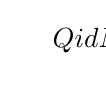
\begin{tikzpicture}
\tikzset{level distance=50pt, sibling distance=1.5pt}
  \Tree [.{$Q$}
    [.{$id$} ]
    [.{$N$}
      [.{$Q$}
        [. \node(q0){$q_0$}; ]
        [. \node(qn){$q_n$}; ]
      ]
      [.{$A$}
        [. \node(a0){$a_0$}; ]
        [. \node(an){$a_n$}; ]
      ]
      [. {$N$}
        [. \node(n0){$n_0$}; ]
        [. \node(nn){$n_n$}; ]
      ]
      [.{$eq$} ]
    ]
    [.{$P$}
      [.{$P$}
        [.{$p_l$} ]
        [.{$p_h$} ]
      ]
      [.{$M$}
        [.{$m_l$} ]
        [.{$m_h$} ]
      ]
      [.{$E$}
        [.{$e_0$} ]
        [.{$e_1$} ]
        [.{$e_2$} ]
        [.{$e_3$} ]
      ]
      [.{$L$}
        [.{$l_s$} ]
        [.{$l_l$} ]
      ]
      [.{$F$}
        [.{$f_n$} ]
        [.{$f_s$} ]
      ]
    ]
    [.{$E$}
      [.{$m$} ]
      [.{$T$}
        [. \node(tl){$t_l$}; ]
        [. \node(th){$t_h$}; ]
      ]
    ]
  ]
\begin{scope}[dashed]
\draw (a0)--(an);
\draw (n0)--(nn);
\draw (q0)--(qn);
\end{scope}
\end{tikzpicture}
\caption[Structure of the query tree for composing searches]
        {Structure of the query tree used for composing searches of
          PIP-DB. Leaf nodes represent properties. Nodes
          with an uppercase name denote compound AND conditionals.}
\label{fig:query-tree}
\end{figure}

% TODO: Example queries


\newpage

%%%%%%%%%%%%%%%%%%%%%%%%%
%% Listing: query-tree %%
%%%%%%%%%%%%%%%%%%%%%%%%%
\lstset{language=clojure}
\begin{lstlisting}[label=lst:query-tree,caption={%
      [Clojure implementation of the query tree]
      Implementation of the query tree in Clojure, from the file
      \texttt{query.clj}. Note the flat query hierarchy and the
      use of the \texttt{for} macro for expanding multivalued
      queries.}]
(AND
 (EQ   {:field "id"            :value id :exact true})
 (for [word q]
   (EQ {:field "Protein-Names" :value word}))
 (for [word q_any]
   (EQ {:field "Protein-Names" :value word}))
 (for [word q_ne]
   (NE {:field "Protein-Names" :value word}))
 (EQ   {:field "Protein-Names" :value q_eq})
 (EQ   {:field "Source"        :value q_s})
 (EQ   {:field "Location"      :value q_l})
 (EQ   {:field "Method"        :value m})
 (EQ   {:field "Sequence-Name" :value seq})
 (GTE  {:field "real_pi_min"   :value pi_l})
 (LTE  {:field "real_pi_max"   :value pi_h})
 (GTE  {:field "real_mw_min"   :value mw_l})
 (LTE  {:field "real_mw_max"   :value mw_h})
 (GTE  {:field "real_temp_min" :value t_l})
 (LTE  {:field "real_temp_max" :value t_h})
 (EQ   {:field "real_ec1"      :value ec1 :numeric true})
 (EQ   {:field "real_ec2"      :value ec2 :numeric true})
 (EQ   {:field "real_ec3"      :value ec3 :numeric true})
 (EQ   {:field "real_ec4"      :value ec4 :numeric true}))
\end{lstlisting}


\subsection{Incorporating BLAST searching}\label{subsec:blast-searching}

One of the extensions to the core search engine suggested by Dr Flower
was to add the ability to perform queries of PIP-DB using Basic Local
Alignment Search Tool (BLAST) searching. NCBI BLAST consists of a
suite of search tools\footnote{BLAST+ executables
  \url{http://blast.ncbi.nlm.nih.gov}.}
which can query a database of proteins sequences in the FASTA format,
allowing users to identify proteins using parts of
sequences. Incorporating BLAST searching in pip-db involved developing
a dynamic dispatcher for the search engine which would invoke the
required BLAST+ executable when needed.

\subsubsection*{Dynamic dispatcher}

Dynamic dispatch is the process by which a polymorphic function
determines which behaviour to use at run time. The process is used
extensively in pip-db, for example, routing request maps to ring
handlers (Section~\ref{subsec:routing}). For searches, the main search
function inspects the search parameters and determines whether a BLAST
search is needed (i.e.\ whether the search parameters include a FASTA
sequence). If a BLAST search is required, then the
\textit{blast/search} function is used to handle the
search. Otherwise, the \textit{db/search} function is used. In both
cases, the results are merged into a results map which contains
auxiliary information such as the number of records which were
searched and the number of matching records. The custom HTTP headers
``x-pip-db-query-terms'' and ``x-pip-db-records'' can be used to
further control the contents of the response map. See
Listing~\ref{lst:search-dispatcher} for the dispatcher implementation.

\newpage

%%%%%%%%%%%%%%%%%%%%%%%%%%%%%%%%
%% Listing: search-dispatcher %%
%%%%%%%%%%%%%%%%%%%%%%%%%%%%%%%%
\lstset{language=clojure}
\begin{lstlisting}[label=lst:search-dispatcher,caption={%
      [Search handler and dynamic dispatcher]
      Search handler and dynamic dispatcher. Accepting a request map,
      the search handler dispatches the appropriate search function
      (line \ref{lst:search-dispatcher-dispatch}), wrapping the
      results into a response map.}]
(defn search [request]
  (let [sequence     ((request :params) "seq")
        blast?       (not (str/blank? sequence))
        params       (request :params)
        headers      (request :headers)
        query-terms? (not (= (headers "x-pip-db-query-terms") "None"))
        records?     (not (= (headers "x-pip-db-records")     "None"))
(*@\label{lst:search-dispatcher-dispatch}@*)        matching-records    (if blast? (blast/search request)
                                       (db/search    request))
        no-records-searched (if blast? (blast/no-of-records)
                                       (db/no-of-records))]
    (merge
     (if records?
       (let [returned-records (take max-no-of-returned-records
                                    matching-records)]
         {:No-Of-Records-Returned  (count returned-records)
          :Records                  returned-records}))
     {:No-Of-Records-Matched       (count matching-records)
      :Max-No-of-Returned-Records   max-no-of-returned-records
      :No-Of-Records-Searched       no-records-searched}
     (if query-terms?
       {:Query-Terms               (dissoc params "seq_name")}))))
\end{lstlisting}


In line~\ref{lst:search-dispatcher-dispatch}, either the
\textit{blast/search} or \textit{db/search} functions are dispatched
to handle the search request, depending on whether it is a BLAST or
non-BLAST search, respectively. Listing~\ref{lst:db-search} shows the
implementation of the \textit{db/search} function for performing
non-BLAST searches.


%%%%%%%%%%%%%%%%%%%%%%%%
%% Listing: db-search %%
%%%%%%%%%%%%%%%%%%%%%%%%
\lstset{language=clojure}
\begin{lstlisting}[label=lst:db-search,caption={%
      [The \textit{db} namespace search function]
      The \textit{db} namespace search function.}]
(defn search [request]
(*@\label{lst:db-search-str}@*)  (let [query-str (params->str (request :params))]
(*@\label{lst:db-search-row}@*)    (map row->record (search-results query-str))))
\end{lstlisting}

The \textit{params->str} function (line~\ref{lst:db-search-str}) is
responsible for serialising a parameter map into a structured query
tree, and serialises it into an SQL select statement. This is used to
generate a vector of SQL record rows which are mapped over the
\textit{row->record} function (line~\ref{lst:db-search-row}),
converting them back into structured YAPS records by post-processing
the data.

The BLAST search function (Listing~\ref{lst:blast-search}) first
executes the \textit{blastp} program with an appropriate environment
and input filtered from the request map
(line~\ref{lst:blast-search-blastp}), and then maps the output of the
program into the function \textit{result->records} which performs a
reverse lookup of the matched sequences and performs repeated database
searches for the matched records using the parameter
map. Listing~\ref{lst:blast-search-wrapper} shows the implementation
of the \textit{results->records} function, showing the functional
composition of the db search function to produce blast search
(line~\ref{lst:blast-search-wrapper-db}).


%%%%%%%%%%%%%%%%%%%%%%%%%%%
%% Listing: blast-search %%
%%%%%%%%%%%%%%%%%%%%%%%%%%%
\lstset{language=clojure}
\begin{lstlisting}[label=lst:blast-search,caption={%
      [The \textit{blast} namespace search function]
      The \textit{blast} namespace search function.}]
(defn search [request]
(*@\label{lst:blast-search-blastp}@*)  (let [results (blast-results ((request :params) "seq"))]
(*@\label{lst:blast-search-map}@*)    (flatten (map #(result->records request %) results))))
\end{lstlisting}


\newpage


%%%%%%%%%%%%%%%%%%%%%%%%%%%%%%%%%%%
%% Listing: blast-search-wrapper %%
%%%%%%%%%%%%%%%%%%%%%%%%%%%%%%%%%%%
\lstset{language=clojure}
\begin{lstlisting}[label=lst:blast-search-wrapper,caption={%
      [BLAST search output processing]
       BLAST search output processing.}]
(defn result->records [request result]
  (let [params  (assoc (request :params) "seq_name" (result :title))
(*@\label{lst:blast-search-wrapper-db}@*)        records (db/search (assoc request :params params))]
    (map #(wrap-blast-result % result) records)))
\end{lstlisting}


\subsection{API and mobile code}\label{subsec:api}

After the implementation of the core search engine component, an API
was designed which would expose the search functionality publicly. The
purpose of a public API is to allow for programmatic public
interaction with the search engine. This allows users to write their
own clients for performing searches. Communications with the public
API uses the JSON file format transmitted over HTTP. The reason for
using JSON is that it is a lightweight data encoding which is widely
and simply supported in a number of programming languages, and
translates easily to and from the map structures which are used
internally within the pip-db web server. All that was required to
implement the public API was to assign ring handlers which wrap the
internal search functions into JSON responses, shown in
Listing~\ref{lst:api-handlers}.

The public API offers benefits to software developers who intend to
develop their own pip-db clients. Additionally, it also aids in
development of the core website itself. By having a solid public API
which is capable of interacting with the search engine, it is possible
to avoid having to perform the dynamic generation of HTML for search
results within the web server, and instead transmit mobile JavaScript
scripts which interact with the public API and generate the required
HTML on the client side. Doing so means that the public API is the
only entry point for the search engine, which has many
advantages. Firstly, it creates a simpler project, since it reduces
the number of the APIs. Both internal and external clients use the
same consistent API. This improves maintainability, as there is only
one point of change for modifications, and it reduces the code
size. Using mobile code also reduces the bandwidth load on the server,
as transmitted JavaScript can be cached by web clients, requiring only
JSON search results to be transmitted. This increases the throughput
of the server by offloading the computational expense of generating
HTML from the web server to the client browser, and uses the standard
distributed application practise of balancing computation across all
nodes in a system, not relying on the central web server node to
preform all of the computation, leading to performance bottlenecks.

The size of the client side vs.\ web server code bases are indicative
of the amount of computation that is performed on each side. The
pip-db web server consists of 1,882 lines of Clojure LISP, and the
line count for client side scripts is only marginally lower at
1,713. This indicates the balance between server-side and client-side
computation. The public API also enables asynchronous AJAX
communications with the search engine, a feature which is exploited
extensively in the usability features described in
Section~\ref{subsec:ux}.\\


%%%%%%%%%%%%%%%%%%%%%%%%%%%
%% Listing: api-handlers %%
%%%%%%%%%%%%%%%%%%%%%%%%%%%
\lstset{language=clojure}
\begin{lstlisting}[label=lst:api-handlers,caption={%
      [API ring handler implementations]
       API ring handler implementations, taken from \texttt{api.clj}.}]
(defn s [request]
  (util/json-response (search/search request)))

(defn r [request]
  (util/json-response (search/search (util/remap-id-param request))))
\end{lstlisting}


\subsection{API-enabled search engine usability}\label{subsec:ux}

As described in Section~\ref{subsec:user-centred-design}, a
human-centred approach was adopted for the design of the
website. Through consistent interaction with potential users and the
evaluation of common use cases, a number of attempts to innovate the
user experience for bioinformatics search engines were made. For the
search page, a combination of mobile code and the public API was used
to implement two features to streamline the process of entering
complex searches: the first is context sensitive Autocompletion of
fields using a dedicated API, and the second is a widget which
indicates the number of results will be returned by a given
search. Figure~\ref{fig:search-sequence} shows how a client browser
interacts with these APIs when the user fills in a search form.


%%%%%%%%%%%%%%%%%%%%%%%%%%%
% Figure: search-sequence %
%%%%%%%%%%%%%%%%%%%%%%%%%%%
\begin{figure}[H]
\centering
\begin{sequencediagram}
% Client side
\newthread[white]{user}{User}
\newinst[2]{browser}{Browser}

% Server side
\newinst[3]{api-ac}{/api/ac}
\newinst{api-s}{/api/s}
\newinst{s}{/s}
\newthread[white]{db}{db}

% AUTOCOMPLETION
\begin{sdblock}{loop}{Autocompletion}
  \begin{call}{user}{Keystroke}{browser}{Suggestions}
    \begin{call}{browser}{Field value}{api-ac}{Results map}
      \begin{call}{api-ac}{Lookup}{db}{Results}
      \end{call}
    \end{call}
  \end{call}
\end{sdblock}

% RESULTS INDICATOR
\begin{sdblock}{loop}{Results indicator}
  \begin{call}{user}{Modify form}{browser}{No of results}
    \begin{call}{browser}{Form values}{api-s}{Results map}
      \begin{call}{api-s}{Search}{db}{Results}
      \end{call}
    \end{call}
  \end{call}
\end{sdblock}

% FORM SUBMISSION
\begin{call}{user}{Submit form}{browser}{Results page}
  \begin{call}{browser}{Form values}{s}{Results map}
    \begin{call}{s}{Search}{db}{Results}
    \end{call}
  \end{call}
\end{call}
\end{sequencediagram}
\caption[Search form sequence diagram]{Search form sequence
  diagram. The instances \texttt{/api/ac}, \texttt{/api/s}, and
  \texttt{/s}, represent the public web services available at those
  locations. Communication from the browser to those services takes
  the form of asynchronous HTTP GET requests.}
\label{fig:search-sequence}
\end{figure}


\newpage
\section{Website design and usage}\label{sec:website-design}

This section contains an annotated visual overview of the design of
the pip-db website, and its usage instructions.

\vspace{1.5cm}


%%%%%%%%%%%%%%%%%%%%
%% Figure: pip-db %%
%%%%%%%%%%%%%%%%%%%%
\begin{figure}[H]
\centering
    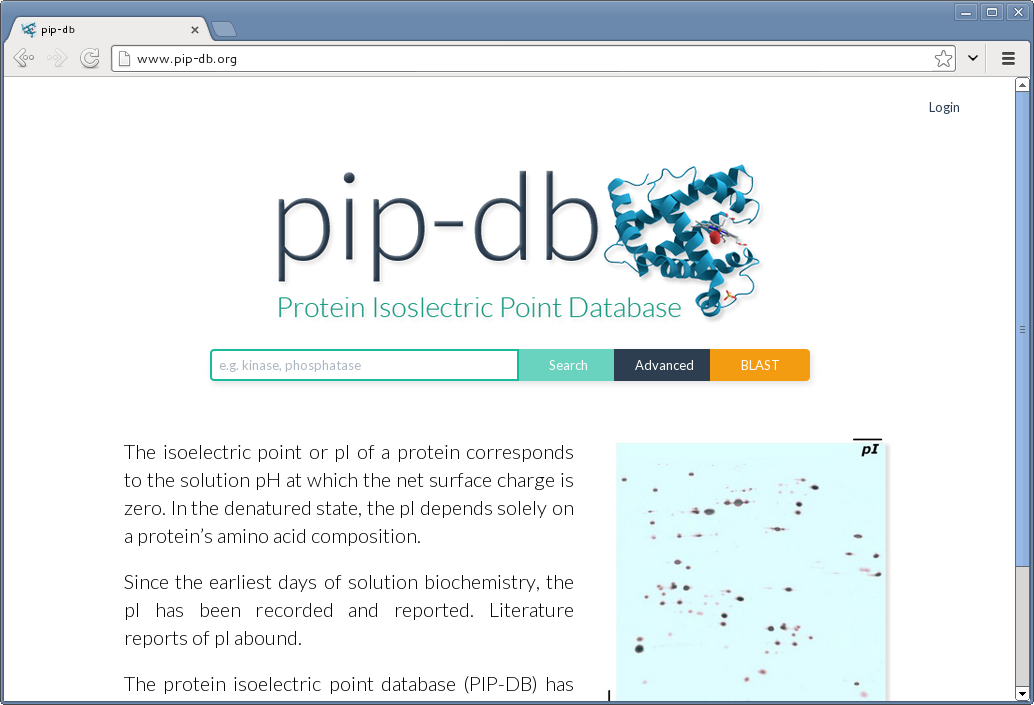
\includegraphics[width=0.82\textwidth]{assets/pip-db}
\caption[pip-db homepage]
        {The pip-db homepage. This provides the main entry point into
          the website. Users may perform basic protein name queries,
          and navigate to the advanced search and BLAST search
          pages. The copy is text provided by Dr Flower to explain the
          purpose of PIP-DB and to provide scientific context and
          background for the data.}
\label{fig:pip-db}
\end{figure}


%%%%%%%%%%%%%%%%%%%%%%%%%%%%%
%% Figure: pip-db-advanced %%
%%%%%%%%%%%%%%%%%%%%%%%%%%%%%
\begin{figure}[H]
\centering
    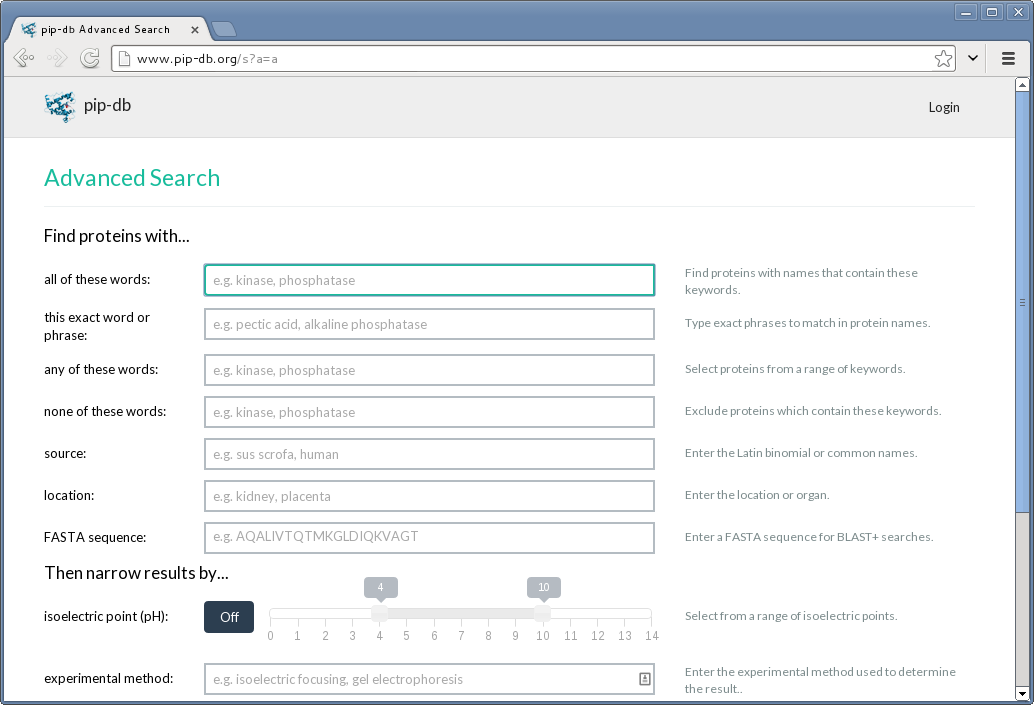
\includegraphics[width=0.82\textwidth]{assets/pip-db-advanced}
\caption[pip-db advanced search page]
        {The pip-db advanced search page. This page allows users to
          query the database using a combination of different
          properties, including protein name keyword matching, and
          numerical properties such as temperature and pI.}
\label{fig:pip-db-advanced}
\end{figure}


%%%%%%%%%%%%%%%%%%%%%%%%%%%%%%%%%
%% Figure: pip-db-autocomplete %%
%%%%%%%%%%%%%%%%%%%%%%%%%%%%%%%%%
\begin{figure}[H]
\centering
    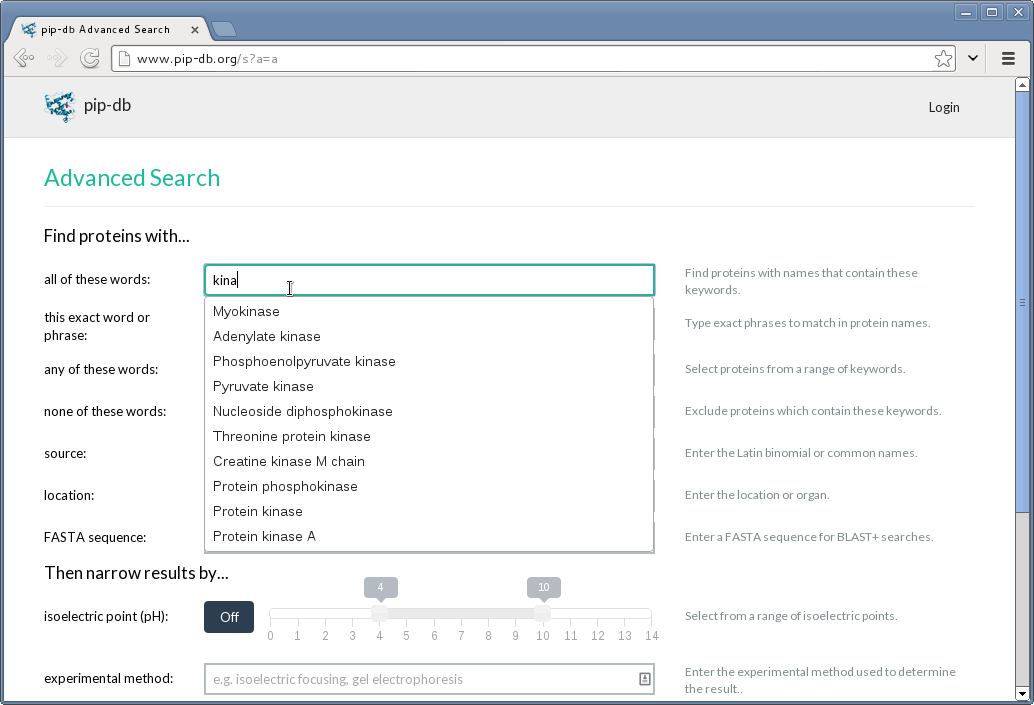
\includegraphics[width=0.82\textwidth]{assets/pip-db-autocomplete}
\caption[Autocompletion suggestions in pip-db]
        {Autocompletion suggestions on the advanced search page for
          the term \textit{kina}. The autocompletion API uses
          frequency analysis of the most common terms in the database
          to provide appropriate suggestions, so that the most
          frequently used matching terms are suggested first.}
\label{fig:pip-db-autocomplete}
\end{figure}


%%%%%%%%%%%%%%%%%%%%%%%%%%%%%%%%%%%%%%
%% Figure: pip-db-results-indicator %%
%%%%%%%%%%%%%%%%%%%%%%%%%%%%%%%%%%%%%%
\begin{figure}[H]
\centering
    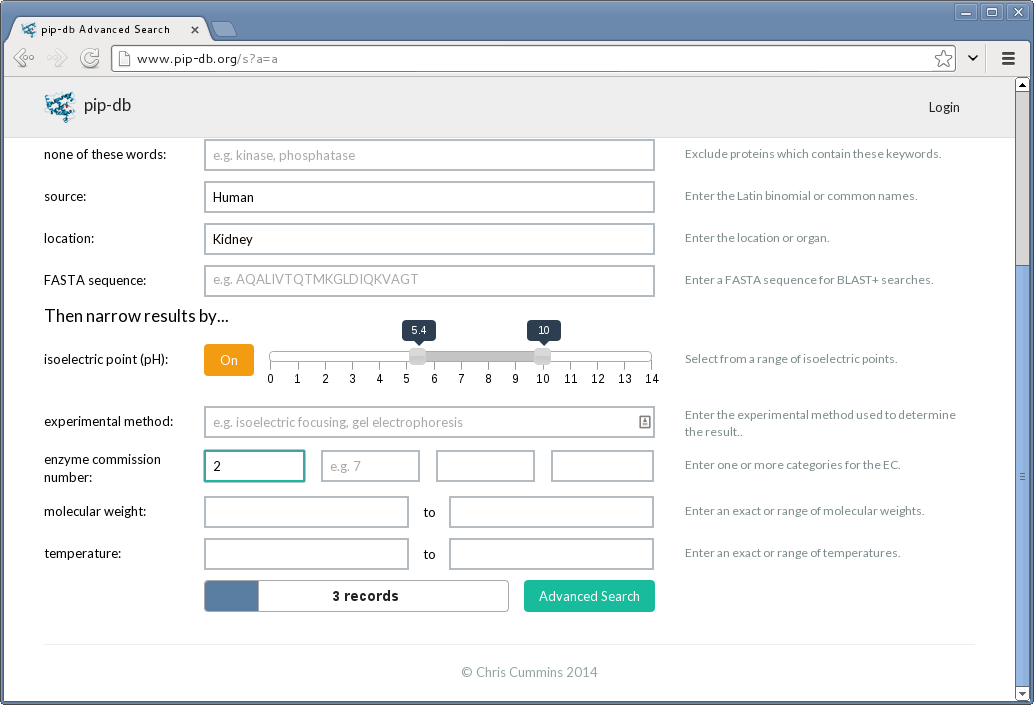
\includegraphics[width=0.82\textwidth]{assets/pip-db-results-indicator}
\caption[pip-db results indicator]
        {The pip-db results indicator on the advanced search page. The
          results indicator shows the number of records which match
          the current search query, and is updated dynamically as the
          user fills out the form. The screenshot shows that 3 records
          will be returned for the current search terms. Also visible
          is the use of a sliding range input widget for specifying a
          range of pI values to search.}
\label{fig:pip-db-results-indicator}
\end{figure}


%%%%%%%%%%%%%%%%%%%%%%%%%%%%
%% Figure: pip-db-results %%
%%%%%%%%%%%%%%%%%%%%%%%%%%%%
\begin{figure}[H]
\centering
    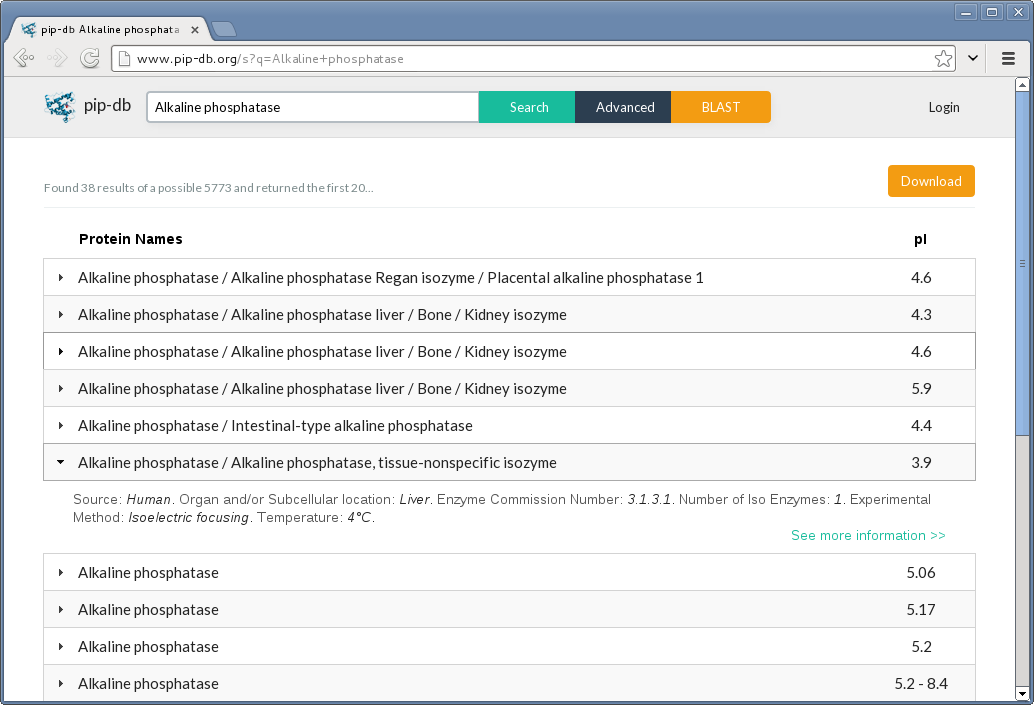
\includegraphics[width=0.82\textwidth]{assets/pip-db-results}
\caption[pip-db results page]
        {The pip-db search results page for the search term
          \textit{Alkaline phosphatase}. The search results page lists
          the protein names and pI of each matching record. If the
          user clicks on a record, further information about the
          record is revealed. Clicking the ``See more information''
          link will then redirect the user to that specific record's
          page. There is a button to download the search results in
          CSV or JSON formats.}
\label{fig:pip-db-results}
\end{figure}


%%%%%%%%%%%%%%%%%%%%%%%%%%%
%% Figure: pip-db-record %%
%%%%%%%%%%%%%%%%%%%%%%%%%%%
\begin{figure}[H]
\centering
    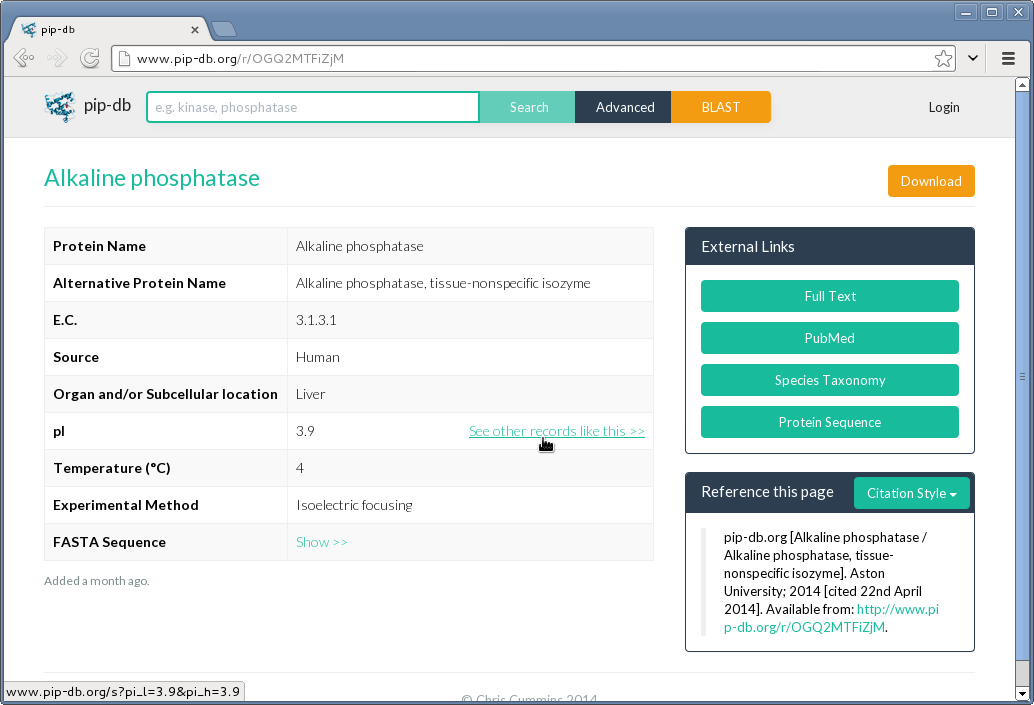
\includegraphics[width=0.82\textwidth]{assets/pip-db-record}
\caption[pip-db record page]
        {The pip-db record page, showing an \textit{Alkaline
            phosphatase} entry. The page shows property values, with a
          ``See other records like this'' link for showing records
          with identical property values. Links and cross-references
          to external resources are shown in the top right, along with
          a button to download the record. Beneath that is an
          automatic page reference generator, for the purpose of
          citations.}
\label{fig:pip-db-record}
\end{figure}


%%%%%%%%%%%%%%%%%%%%%%%%%%%%%
%% Figure: pip-db-download %%
%%%%%%%%%%%%%%%%%%%%%%%%%%%%%
\begin{figure}[H]
\centering
    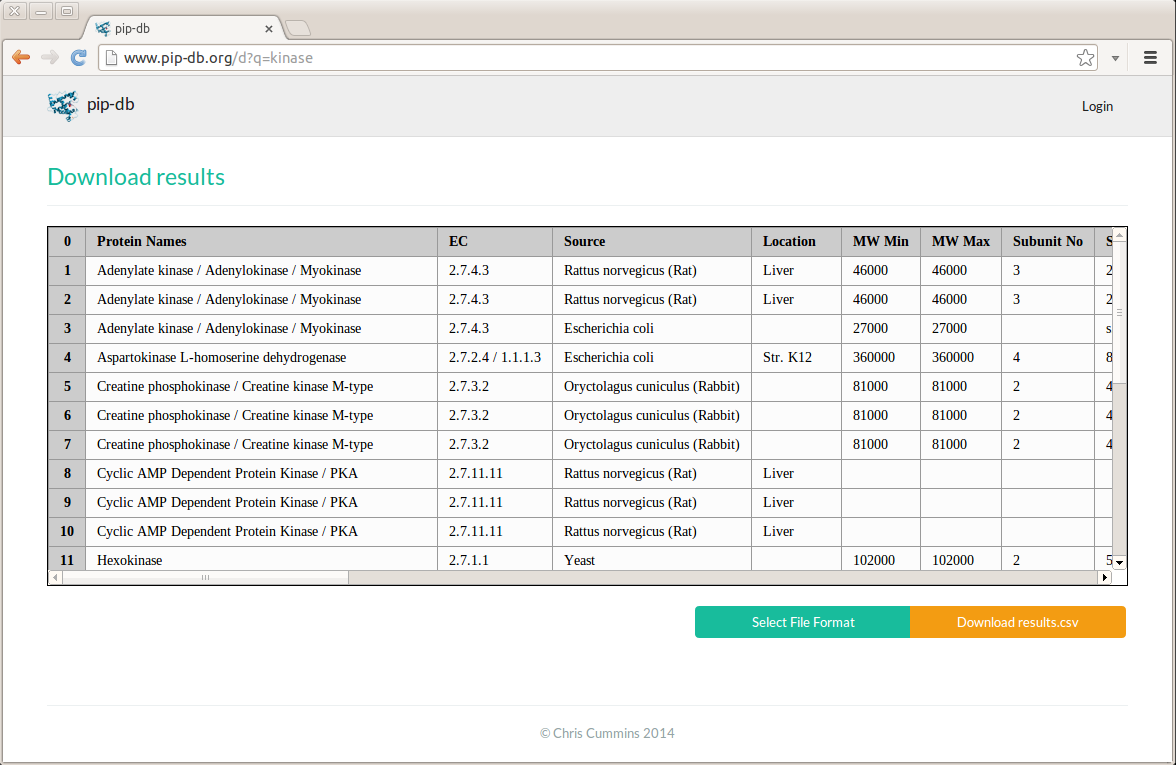
\includegraphics[width=0.82\textwidth]{assets/pip-db-download}
\caption[pip-db download results page]
        {The pip-db download results page, which supports the download
          of search results and individual records in either CSV or
          JSON formats.}
\label{fig:pip-db-download}
\end{figure}
